\section{Part I -- Exact method}

In this section I'll describe the implementation details for the first part of
the exercise, i.e. the one that finds the global optimum thanks to \cplex.

\subsection{Data structures}
Before calling the proper API to solve the optimization problem, the main
procedure of the program has to write down the problem in the \cplex{}
environment.

This goal is indeed accomplished by calling a sub-procedure \texttt{setupLP}
that is accountable for generating variables and constraints: thus, along this
function we need to keep track of the indexes of the variables we declared so
that we are able to refer to them when creating the constraints.

An initial solution could be to inspect how variables are defined and then
re-compute their indexes each time we need to refer to a given variable.

It is easy to see that this approach may lead to poor code quality: if variables
were generated in another procedure and then the incomplete problem was handed
off to another programmer, she would have to look at \textit{how} her colleague
defined the variables (all of this without guarantees that the variables
generation is fixed).

Thus, an (pretty straightforward) alternative solution is to store variables'
indexes in a ``map'' while generating the variables, i.e. an $n$-dimensional
vector where $n$ is the dimension of a certain variable\footnote{if a variable
$x_{i,j}$ is indexed with two factors $i$ and $j$, then the map relative to
$x_{i,j}$ will have two dimensions}.
Therefore, variables and constraints generation are now loosely coupled, which
is clearly a good software engineering discipline: in fact, in the previous
scenario the former programmer will pass the indexes maps to the latter, without
requiring her to know any implementation detail.

\subsection{Variables generation}
In \cplex, before you create the constraints you (reasonably) have to declare
the variables you are going to use. Since in this situation the model is
relatively small, it is (arguably) more important to create it in a more
expressive and clear manner rather than it is to make it efficiently.

For this reason, variables of the sort $x_{i,j}$ and $y_{i,j}$ were defined in
two separated cycles, iterating twice over the range of all $i,j\in{N}$, where
$N$ is the set of holes. Also, I did not taken out from the model the useless
variables $x_{i,i}$, since they cause negligible effort both regarding to
memory space and computing time.

\subsection{Constraints generation}
As it was done for variables, clarity has been chosen over efficiency for
constraints too. Thus, constraints were added in several blocks so anyone can
be able to understand what the program is doing at that line of code by looking
at the comments at the beginning of each block.

\subsection{Sample data generation}
An important point for this part of the assignment is being able to generate
realistic data to make the solver run under different conditions.
Therefore, I thought of creating data in several manners.

\paragraph{Hard-coded values} The simplest way to have sample data to test the
solution was to put fixed input data to the problem, so it was easy to see if
both the problem and the solution given by the program were correct.

The solver was in fact tested against this configuration and other two:

\begin{figure}[h!]
\centering
\begin{tikzpicture}
\foreach \Point in {(0,0), (1.5,0), (1.5,2)}{
  \node at \Point {\textbullet};
}
\end{tikzpicture}
\end{figure}

These points are placed in a classical $3$-$4$-$5$ Pythagorean triple, thus it
is very easy to figure out the problem structure and its solution.

Apart from this simple hard-coded configuration, I have used also two hard-coded
configurations with 12 and 60 nodes, which we were given by the professor.

\paragraph{Random Uniform generation} The second way we can generate sample data
is doing it in a random uniform fashion.

In fact, this generator produces a list of nodes and distances from one node to
every other node.

There are several benefits and drawbacks that come with this approach:

\begin{itemize}
  \item \textbf{Pros}:
  \begin{itemize}
    \item When compared to the hard-coded value, it is easier to generate large
      samples to run the program against;
    \item Compared to the Gerber generation, it is easier to test the
		  efficiency of the program against huge amount of data (i.e., far bigger
			than a realistic drilling problem);
    \item It provides some entropy among several runs, so it is less hard to
      capture the average behaviour of the program against a completely generic
      sample instance.
  \end{itemize}
  \item \textbf{Cons}:
  \begin{itemize}
    \item There is no guarantee on the fact that the generator will provide
      realistic data w.r.t. the domain problem;
    \item It is more complex to use for initial testing of the model compared
      to hard-coded data, since you have to solve manually the problem to be
      sure that it works without errors.
  \end{itemize}
\end{itemize}

\paragraph{Random Grid Uniform generation} The third way we can generate sample
data is doing it in a random uniform fashion within cells of a grid.

In fact, the previous approach did not consider the position of the points in
the PCB (\textit{printed circuit boards}), yielding values which may be really
unrealistic. A more realistic solution relies in dividing the grid into areas
and then distribute a fraction of the holes in each one of them.

The algorithm works as follows:
\begin{enumerate}
	\item the user has to provide, as input, the number of holes $n$, the size
	  multiplier and the number of divisions;
	\item the program generates a board which size is proportional to the holes
		and the specified size;
	\item $n$ holes are scattered across all the board, with a fair distribution
	  among different areas;
	\item the program generates a data file in which distances may be created
		either with the euclidean distance or the Manhattan distance.
\end{enumerate}

\begin{figure}[H]
  \centering
  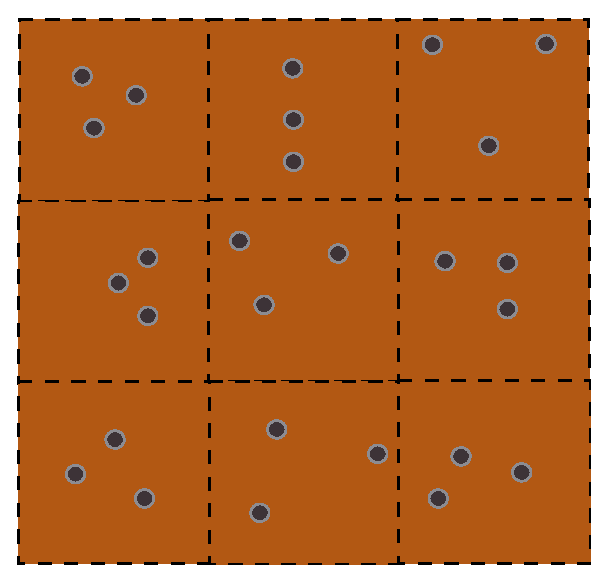
\includegraphics[width=.5\columnwidth]{pics/ru-grid.eps}
  \caption{Graphic representation for Random Grid Uniform}
  \label{fig:ru-grid-sketch}
\end{figure}

Clearly, this new manner of creating instances should be preferred to the
Random Uniform method, which was much more shallow. However, also this methods
relies more on an intuition than on real facts and therefore results generated
by this program should be evaluated with a certain degree of skepticism.

\paragraph{Parsing Gerber files} As it has just been stated in the previous
paragraph random data generation might provide unrealistic samples, which
we would like to be able to filter out in order to capture the average
performance in \textbf{realistic} scenarios.

It turns out that there is a de-facto standard to write files that represents
PCBs. More specifically, in this files we have the information of the positions
of the holes in a PCB among other information (size of the drill, length of the
board, etc.).

Therefore, Mirko Bez and I have implemented a simple Gerber parser to extract
useful information (holes' position) from these files and re-format them so
that they are good sample instances for the solver program.

You can run this program on the browser, where you can feed it with a Gerber
file and it will:
\begin{itemize}
	\item show the holes in a virtual grid;
	\item produce a file containing the euclidean distance between the holes.
\end{itemize}

\begin{figure}[H]
  \centering
  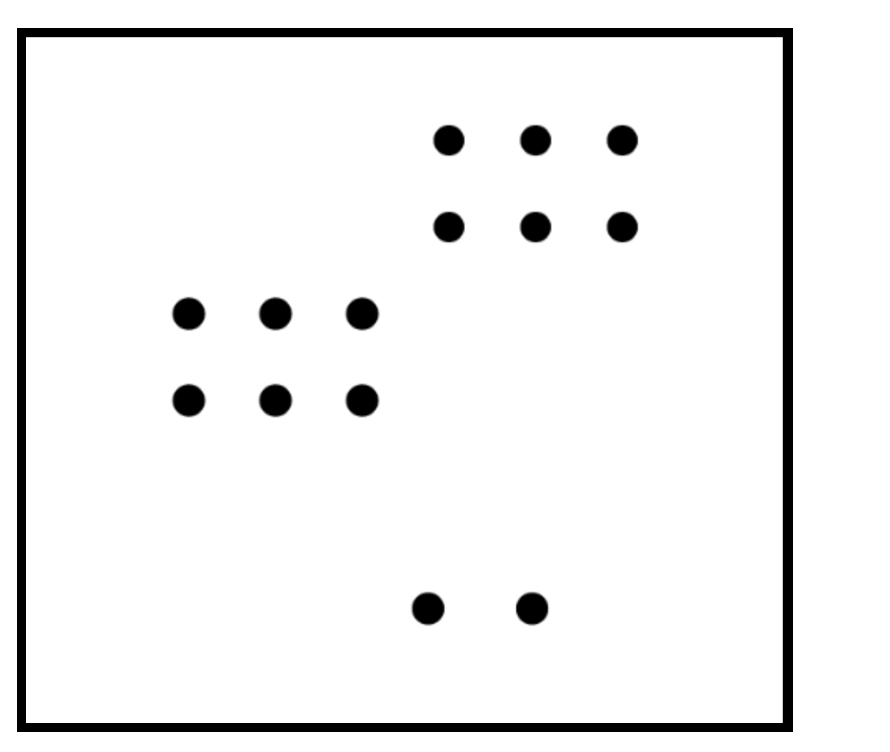
\includegraphics[width=.5\columnwidth]{pics/gerber.eps}
  \caption{Gerber instance sample}
  \label{fig:gerber-instance-pic}
\end{figure}
